\chapter{Building a Cache Simulator}
\label{cha:building_a_cache_simulator}
\par 整个实验分为两个部分,在第一部分中,需要实现一个缓存模拟器。通过valgrind中的lackey工具\footnote{\url{http://valgrind.org/docs/manual/lk-manual.html}}可以得到一个程序几乎所有的内存访问情况,使用如下命令即可获得这些信息:
\inputCodeNoNumberSetLanguage{bash}
\begin{lstlisting}[numbers=none]
linux> valgrind --log-fd=1 --tool=lackey --trace-mem=yes <program>
\end{lstlisting}

\par 一个样例输出如下:
\begin{lstlisting}[numbers=none]
I 0400d7d4,8
 M 0421c7f0,4
 L 04f6b868,8
 S 7ff0005c8,8
\end{lstlisting}

\par 输出的格式为``操作\ 地址,大小'',I表示指令加载,L表示数据加载,S表示数据存储,M表示数据修改,而数据修改应该被当做一次数据加载加上一次数据存储。内存地址以十六进制的形式给出。

\section{实验要求}
\label{sec:shi_yan_yao_qiu_}

\par 此实验要求编写一个Cache模拟器,其输入为Valgrind输出的内存访问轨迹,输出为与csim-ref相同的统计数据。

\par 实验要求:
\begin{itemize}
    \item 模拟器必须在输入参数s、E、b设置为任意值时均能正确工作——即需要使用malloc函数(而不是代码中固定大小的值)来为模拟器中数据结构分配存储空间。
    \item 由于实验仅关心数据Cache的性能,因此模拟器应忽略所有指令cache访问(即轨迹中“I”起始的行)
    \item 假设内存访问的地址总是正确对齐的,即一次内存访问从不跨越块的边界——因此可忽略访问轨迹中给出的访问请求大小
    \item main函数最后必须调用printSummary函数输出结果,并如下传之以命中hit、缺失miss和淘汰/驱逐eviction的总数作为参数:
\end{itemize}

\par 在编写完成后,使用test-csim程序进行测试以及评分。Cache模拟器使用的策略应为LRU替换策略。

\section{实验设计}
\label{sec:shi_yan_she_ji_}

\subsection{总体设计}
\label{sub:zong_ti_she_ji_}

\par 需要修改的文件为csim.c。由于已经给出了框架,首先观察框架中的代码,其中包含以下函数:
\inputCodeSetLanguage{c}
\begin{lstlisting}
accessData(mem_addr_t addr)
freeCache()
initCache()
main(int argc,char * argv[])
printUsage(char * argv[])
replayTrace(char * trace_fn)
\end{lstlisting}

\par 根据函数名和注释可以得知,initCache和freeCache用于初始化和释放cache,printUsage用于打印帮助信息,而replayTrace则直接被主函数调用并调用accessData来模拟Cache的替换过程。而需要修改的函数就是accessData函数。

\par 接下来观察Cache是如何在C语言中被组织并模拟的。首先,文件中定义了如下的结构,来描述cache line,并定义其指针以及指针的指针分别为cache set和cache。
\begin{lstlisting}
typedef struct cache_line {
    char valid;
    mem_addr_t tag;
    unsigned long long int lru;
}
typedef cache_line_t *cache_set_t;
typedef cache_set_t *cache_t;
\end{lstlisting}

\par 而通过initCache中的初始化过程可以得知,文件中描述了一个如图\ref{fig:cacheStructure}所示的cache:

\begin{figure}[htb]
    \centering
    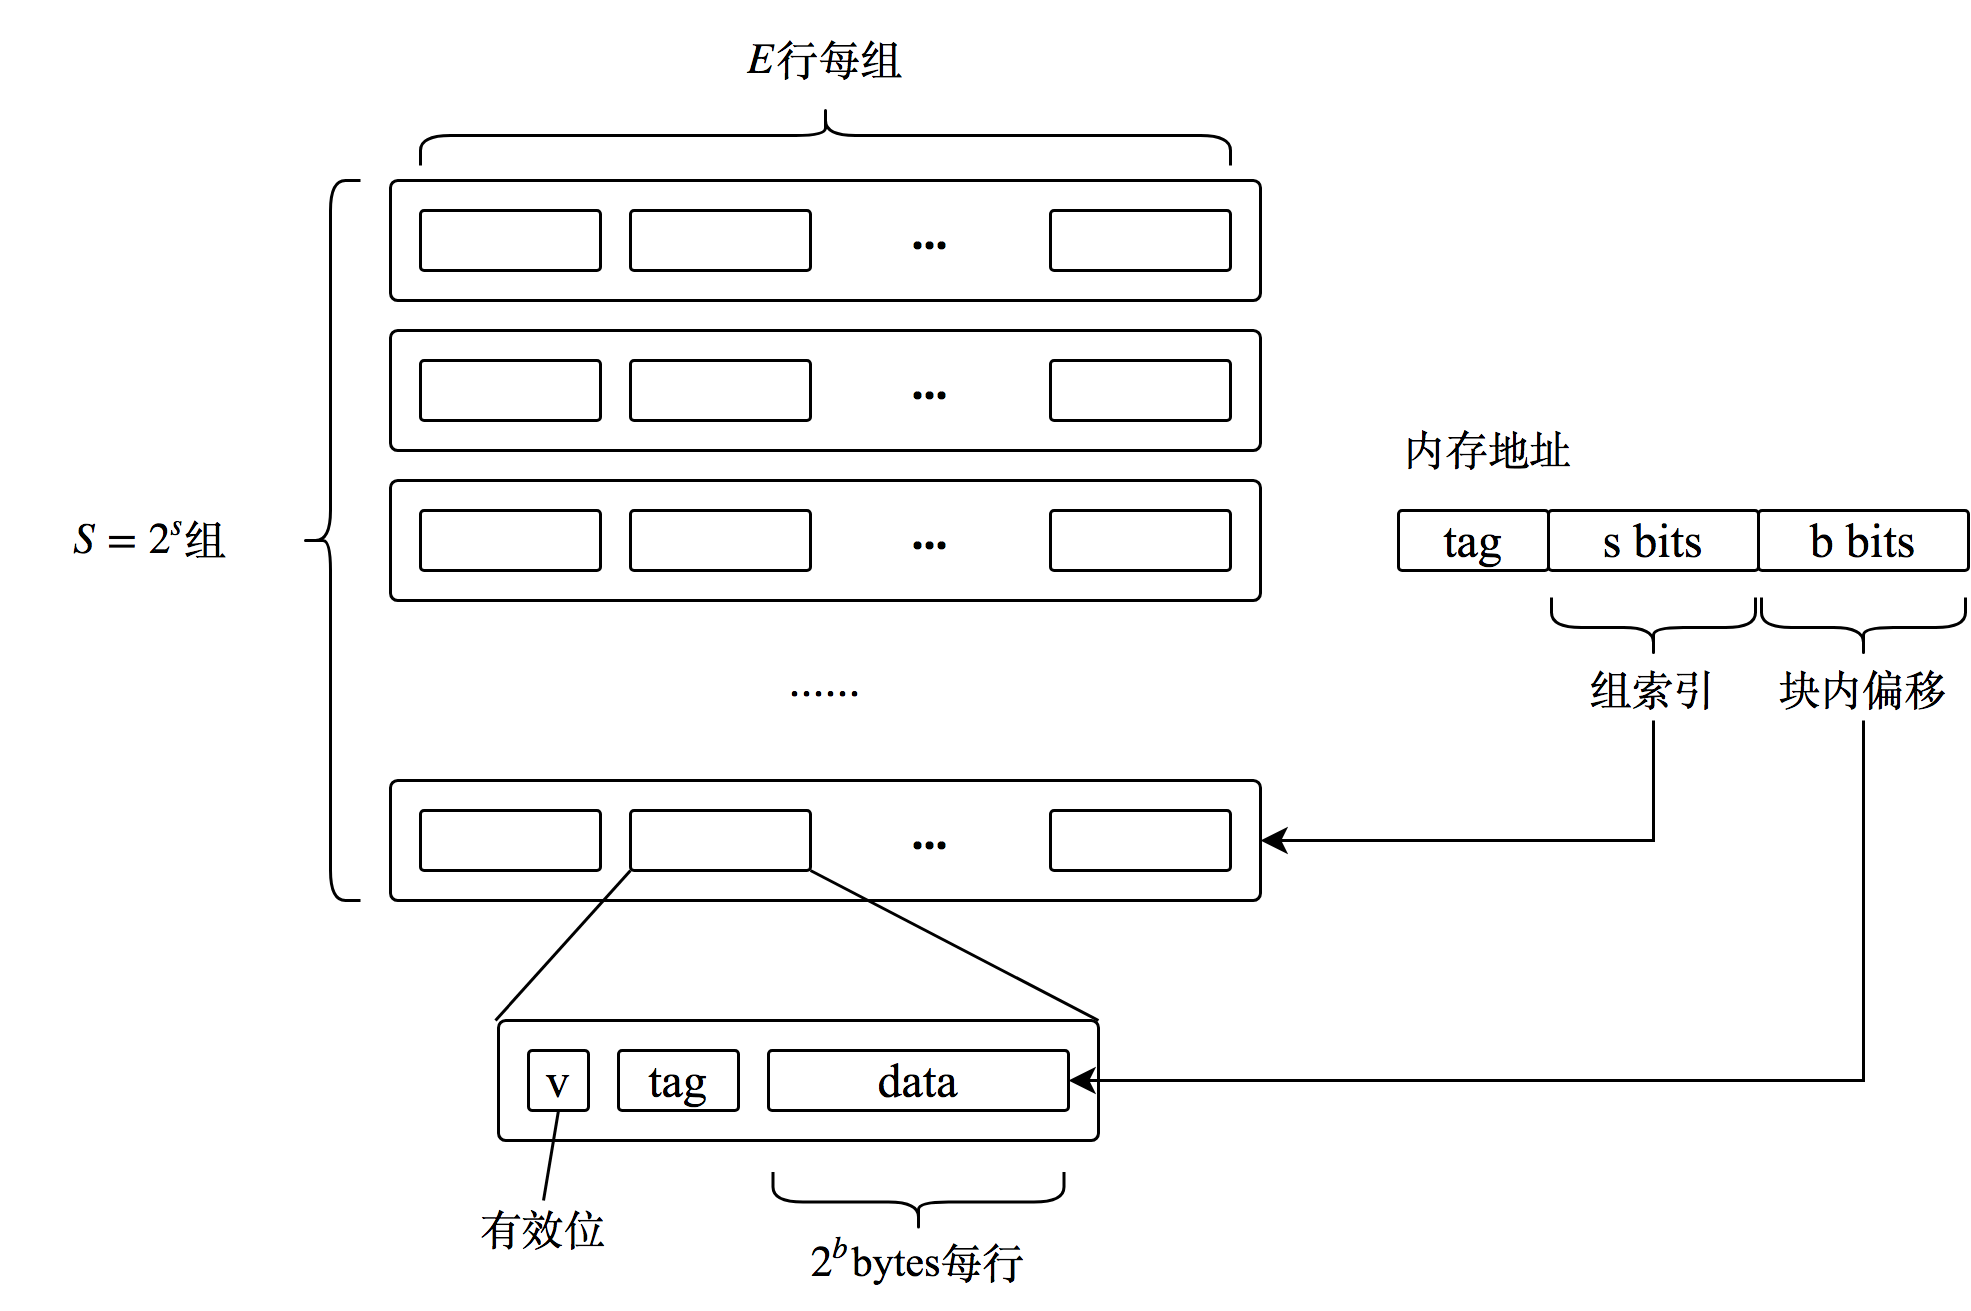
\includegraphics[width=0.72\linewidth]{cacheStructure.png}
    \caption{Cache 结构}
    \label{fig:cacheStructure}
\end{figure}
\FloatBarrier

\par 了解模拟cache在内存中的结构后,每一次的内存访问过程如下:首先判断此内存地址是否能够在对应位置cache hit,如果cache hit则将hit计数加一,否则判定为cache miss,将miss计数加一,然后判断是否需要替换。如果需要替换则按照LRU规则进行替换,然后将eviction计数加一。由于cache line是以数组的形式存在于内存中的,因此在实现LRU的队列结构的时候需要注意对于结构体中lru字段的操作。

\subsection{详细设计}
\label{sub:xiang_xi_she_ji_}
\par 接下来根据LRU的替换规则设计accessData中具体的cache替换流程。首先,根据传入的地址计算组索引以及tag,并根据组索引获得cache组。接下来对于组中的所有cache line进行遍历,若某一个cache line的tag字段与事先计算的tag字段相等,则增加一次cache hit计数,然后更新此cache set中所有cache line的lru字段。若遍历完成都没有cache hit,则一定出现了cache miss,此时将cache miss计数加一。但此时依然需要分类讨论:若此cache set未被填满,则不需要进行替换,直接将新的记录插入cache set中并更新所有cache line的lru字段,否则还需要进行cache替换。替换方法为:首先遍历次cache set中所有的cache line,找出其中lru值最大的cache line(存在时间最长的),将其替换为新的地址后更新其他所有cache line的lru字段。具体的替换流程如图\ref{fig:cacheSub}所示。

\begin{figure}[htb]
    \centering
    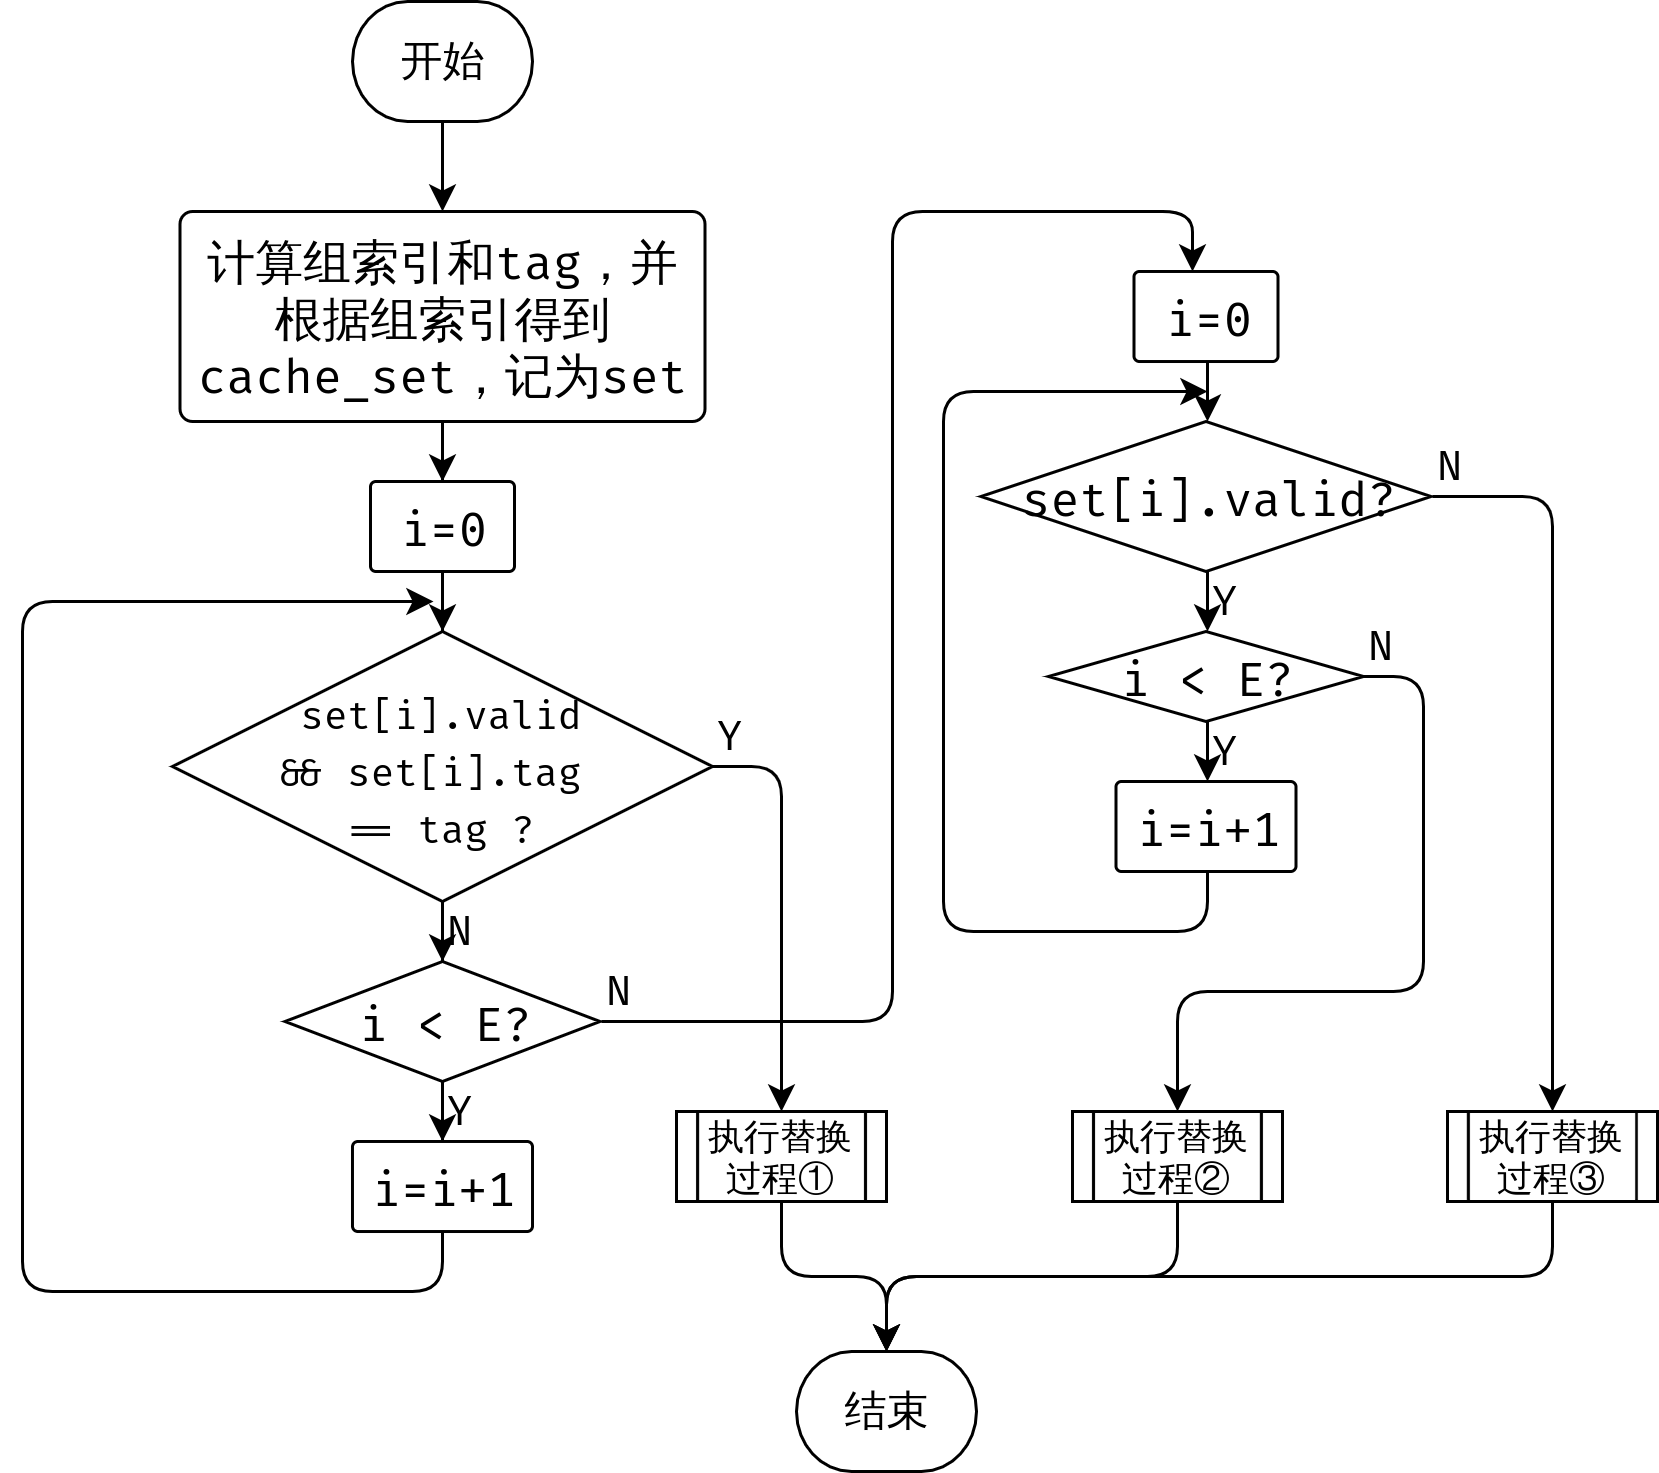
\includegraphics[width=0.7\linewidth]{cacheSub.png}
    \caption{cache更新流程}
    \label{fig:cacheSub}
\end{figure}

\par 在上述三种不同的情况中,三种lru的更新方法是不同的:在cache hit时,遍历所有cache line,将lru字段小于命中的cache的lru字段值,并且valid字段为1的所有cache line的lru值加一,然后将命中的cache line的lru值置为0。
\par 在cache miss但未发生cache eviction时,首先遍历所有cache line,找出第一个valid字为0的cache line,将这一cache line的valid字段置为1,lru字段置为0并将其他所有valid字段为1的cache line的lru值加一。
\par 若出现cache miss eviction,则遍历所有cache line,找出lru值最大的cache line,将其lru值置为0并将这一cache set中其他所有cache line的lru值加一。则这三种替换过程如\ref{fig:cacheSub123}所示。

\begin{figure}[htb]
    \centering
    
\includegraphics[width=0.9\linewidth]{cacheSub123.png}
    \caption{三种情况下的cache替换过程}
    \label{fig:cacheSub123}
\end{figure}

\par 除了上述对于核心部分的设计之外,还需要考虑其他的部分:题目要求实现与csim-ref完全相同的功能,而csim-ref的参数可以指定-h、-v、-s、-E、-b、-t。其中-h在所给出的代码框架中已经得以实现,而-s、-E、-b、-t全部是为核心部分的cache模拟提供支持的。-v参数则需要添加额外的实现。使用-v参数得到的一个样例输出如下:
\inputCodeNoNumberSetLanguage{bash}
\begin{lstlisting}
L 10,1 miss
M 20,1 miss hit
L 22,1 hit
S 18,1 hit
L 110,1 miss eviction
L 210,1 miss eviction
M 12,1 miss eviction hit
hits:4 misses:5 evictions:3
\end{lstlisting}

\par 从输出中可以看出,-v对于除了I型指令之外的内存操作均进行了输出,输出格式与valgrind的输出格式类似,但在每行后面添加了cache hit/miss/eviction的情况。

\section{实验过程}
\label{sec:shi_yan_guo_cheng_}

\subsection{实验环境}
\label{sub:shi_yan_huan_jing_}
\begin{table}[htb]
    \centering
    \caption{实验环境配置}
    \label{tab:label}
    \begin{tabular}{r l}
        \toprule
        操作系统        & Archlinux x64 2018-04-11 更新\\
        编译器          & gcc 7.3.1 \\
        Makefile管理器  & gnu make 4.2.1 \\
        内存调试工具    & valgrind 3.13.0 \\
        版本管理工具    & git 2.17.0 \\
        \bottomrule
    \end{tabular}
\end{table}

\subsection{详细步骤}
\label{sub:shi_yan_guo_cheng_}

\par 有了上述设计后,代码的实现就较为容易了。首先,补全freeCache程序中的代码。根据initCache中的代码可知源程序是在cache这一二维数组的两个维度进行了分配,而从逻辑上可以推断出,在整个程序的运行过程中不需要对于内存进行新的分配,因此,在freeCache时只需要对应的将initCache中分配的内存逐个释放即可。实现的代码如下:
\inputCodeSetLanguage{c}
\begin{lstlisting}
void freeCache() {
    int i;
    for (i = 0; i < S; ++i)
        free(cache[i]);
    free(cache);
}
\end{lstlisting}

\par 接下来实现核心部分代码,也就是accessData模拟cache更新这一部分。首先通过如下代码计算组编号以及tag值,并根据组编号获得cache组。
\begin{lstlisting}
mem_addr_t set_index = (addr >> b) & set_index_mask;
mem_addr_t tag = addr >> (s + b);
cache_set_t cache_set = cache[set_index];
\end{lstlisting}

\par 然后对于cache set进行第一次遍历。在每一次循环中,对于是否命中进行判断,判断的依据为valid是否为1且tag是否与当前内存地址的tag相等。若命中则增加命中计数并进行上述替换过程1,然后直接在返回。此外,还需要注意对于-v参数的支持:如果verbosity flag为1,则需要输出``hit''提示。
\begin{lstlisting}
for (i = 0; i < E; ++i) {
        /* hit */
        if (cache_set[i].valid && cache_set[i].tag == tag) {
            if (verbosity)
                printf("hit ");
            ++hit_count;

            /* update entry whose lru is less than the current lru (newer) */
            for (int j = 0; j < E; ++j)
                if (cache_set[j].valid && cache_set[j].lru < cache_set[i].lru)
                    ++cache_set[j].lru;
            cache_set[i].lru = 0;
            return;
        }
    }
}
\end{lstlisting}

\par 如果上述循环执行完成而没有返回,表明没有发生cache hit,因此使用以下代码将miss技术加一,并在verbosity flag为1时打印``miss''提示。
\begin{lstlisting}
if (verbosity)
    printf("miss ");
++miss_count;
\end{lstlisting}

\par 接下来需要分情况讨论是否会发生cache eviction。经过考虑后发现,可以将不发生eviction情况下寻找最大lru条目的过程与发生eviction情况下寻找第一个invalid cache line的过程合并在同一个循环中,以提高cache模拟器的性能,合并后的循环如下:
\begin{lstlisting}
int j, maxIndex = 0;
unsigned long long maxLru = 0;
for (j = 0; j < E && cache_set[j].valid; ++j) {
    if (cache_set[j].lru >= maxLru) {
        maxLru = cache_set[j].lru;
            maxIndex = j;
        }
    }
}
\end{lstlisting}

\par 在上述循环结束后,通过$j$的值来判断是否发生了cache eviction。由于上述循环在遇到invalid cache line时会跳出,因此当$j$小于E时表明未发生cache eviction。也就是说,如果发生cache eviction,则$j==E$一定成立。因此通过以下代码进行cache的更新。
\begin{lstlisting}
if (j != E) {
    for (int k = 0; k < E; ++k)
        if (cache_set[k].valid)
            ++cache_set[k].lru;
    cache_set[j].lru = 0;
    cache_set[j].valid = 1;
    cache_set[j].tag = tag;
} else {
    if (verbosity)
        printf("eviction ");
    ++eviction_count;
    for (int k = 0; k < E; ++k)
        ++cache_set[k].lru;
    cache_set[maxIndex].lru = 0;
    cache_set[maxIndex].tag = tag;
}
\end{lstlisting}

\par 在上述代码中,$j\neq E$部分为不发生eviction的情况,$j==E$的部分为发生eviction的情况,分别按照章节\ref{sub:xiang_xi_she_ji_}中的方法进行cache的更新。

\par 在accessData中核心部分的代码完成后,需要完成replayTrace中的代码调用accessData完成对于内存访问过程中cache变化的模拟。使用fscanf读入每一行,然后根据访问类型进行对于accessData的调用:忽略I型访问,对于L型和S型访问调用accessData一次,而对于M型访问调用accessData两次,此外还需要注意verbosity flag对于输出的影响。代码如下:
\begin{lstlisting}
while (fscanf(trace_fp, " %c %llx,%d", buf, &addr, &len) > 0) {
    if (verbosity && buf[0] != 'I')
        printf("%c %llx,%d ", buf[0], addr, len);
    switch (buf[0]) {
        case 'I':
            break;
        case 'L':
        case 'S':
            accessData(addr);
            break;
        case 'M':
            accessData(addr);
            accessData(addr);
            break;
        default:
            break;
    }
    if (verbosity && buf[0] != 'I')
        putchar('\n');
}
\end{lstlisting}

\par 至此,所有需要填写的代码已补充完成。

\subsection{测试与分析}
\label{sub:jie_guo_fen_xi_}

\par 对于完成的代码进行测试:首先使用make对代码进行编译,然后直接运行./test-csim命令。实验的测试程序给出的测试样例如表\ref{tab:example}所示,其输出结果如图\ref{fig:result1}所示。

\begin{center}
    \captionof{table}{测试样例}
    \label{tab:example}
    \begin{longtable}{r c c c c c c}
        \toprule
        \multicolumn{1}{c}{\textbf{测试文件}} &
        \multicolumn{1}{c}{\textbf{组索引位数 s}} &
        \multicolumn{1}{c}{\textbf{关联度 E}} &
        \multicolumn{1}{c}{\textbf{块偏移位数 b}} &
        \multicolumn{1}{c}{\textbf{hit}} &
        \multicolumn{1}{c}{\textbf{miss}} &
        \multicolumn{1}{c}{\textbf{eviction}}            \\
        \cmidrule(lr){1-1} \cmidrule(lr){2-4} \cmidrule(lr){5-7}
        yi2.trace   & 1 & 1 & 1 & 9      & 8     & 6     \\
        yi.trace    & 4 & 2 & 4 & 4      & 5     & 2     \\
        dave.trace  & 2 & 1 & 4 & 2      & 3     & 1     \\
        trans.trace & 2 & 1 & 3 & 167    & 71    & 67    \\
        trans.trace & 2 & 2 & 3 & 201    & 37    & 29    \\
        trans.trace & 2 & 4 & 3 & 212    & 26    & 10    \\
        trans.trace & 5 & 1 & 5 & 213    & 7     & 0     \\
        long.trace  & 5 & 1 & 5 & 265189 & 21775 & 21743 \\
        \bottomrule
    \end{longtable}
\end{center}

\begin{figure}[htb]
    \centering
    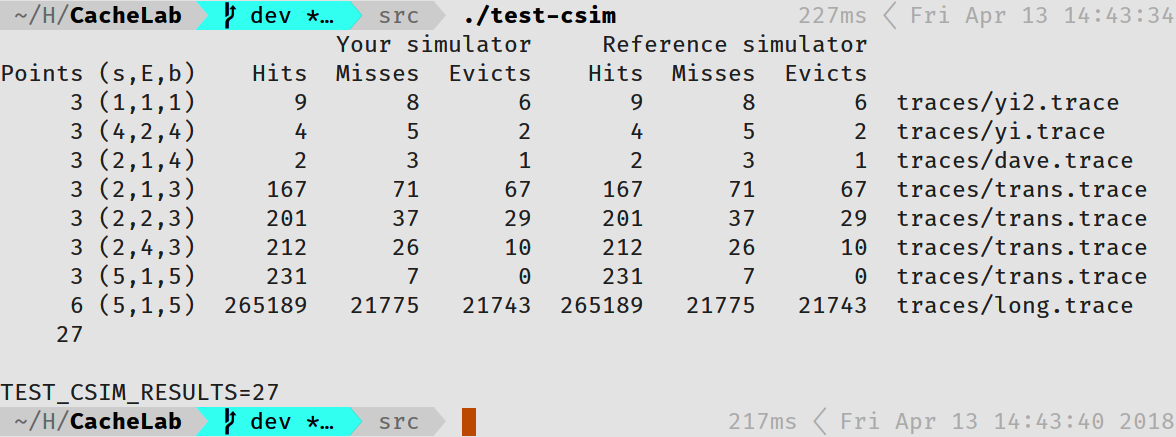
\includegraphics[width=0.8\linewidth]{result1.png}
    \caption{test-csim输出结果}
    \label{fig:result1}
\end{figure}

\par 从图中可以看出,所有的测试通过。接下来对于-v选项进行测试。首先对于yi.trace的进行测试,然后对比处理其他trace文件的输出与csim-ref处理相同文件的输出。运行的结果如\ref{fig:result2}所示。

\begin{figure}[htb]
    \centering
    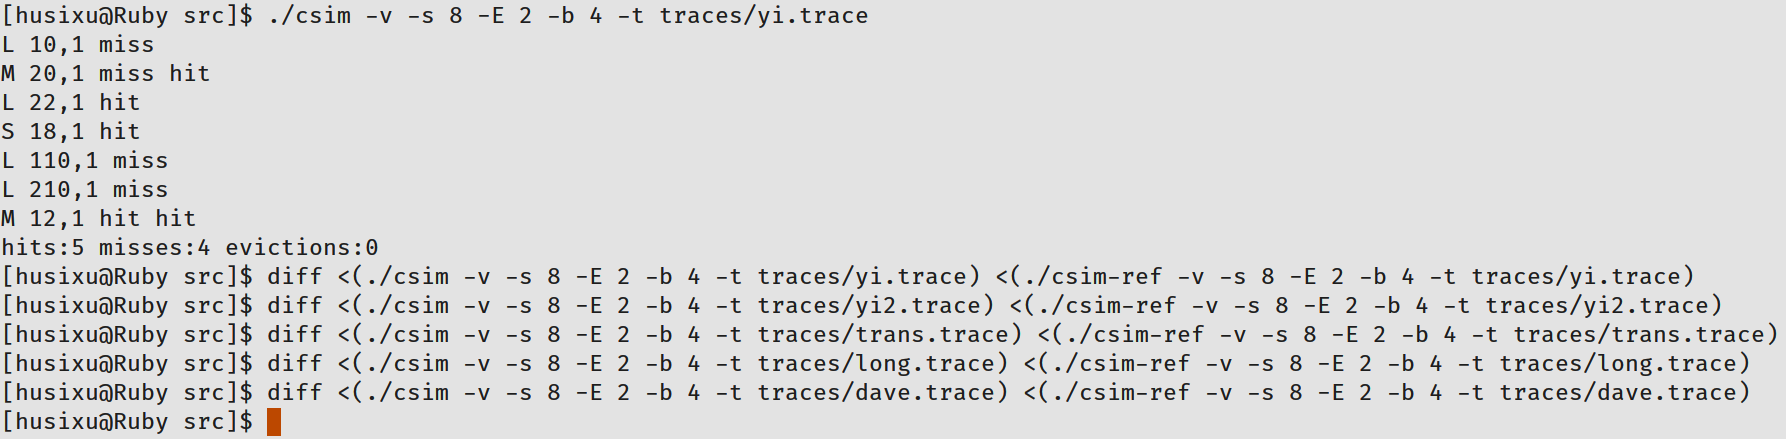
\includegraphics[width=0.95\linewidth]{result2.png}
    \caption{对于-v选项的测试}
    \label{fig:result2}
\end{figure}

\par 可以看出,csim的输出与csim-ref的输出完全相同。至此,所有的测试完成,csim能够完全复现csim-ref的功能。


